\section{Introduction}\label{sec:intro}

We live in a world that has seen a generation of technological revolutions;
from wired to wireless communications, immovable to mobile machines, large
sized to hand-held devices. Today, we are witnessing what can be deemed as the
next phase of mobile revolution through {\em wearable computers}. Research in
wearable computers can be dated back to as early as 1980s when Steve Mann
developed a prototype heads-up-display goggles~\cite{mann1997wearable}. Thanks to the
advances in hardware miniaturization technology, cheap sensors/processor
chips, and low-power sensing/computing, today, wearables are available
off-the-shelf and have almost become an integral part of human
lives~\cite{googleglass,smartwatch,fitbit}.

%This is clearly evident from the surge in the number and types of wearables
%that are commercially available -- ranging from smart glasses, smart
%necklaces, smart wristbands, to smart watches.
The surge in wearables is clearly seen commercially through the array of
smart wearable devices seeping fast into the market. Research on wearables has
actively picked up and is progressing over the day. Keeping in mind the
resource limitations on wearable computers research so far has primarily
been addressing three key optimization parameters in
design: size, energy and cost. With the onset of proliferation of wearable
devices, in the recent times the aspect of security and privacy have also been
adding key concerns to wearable computer usage.
A solution for safeguarding the security and privacy of user's data on the
wearable device is only effective as long as the device itself is
authenticated to the right user/owner.

\begin{figure}
\centering
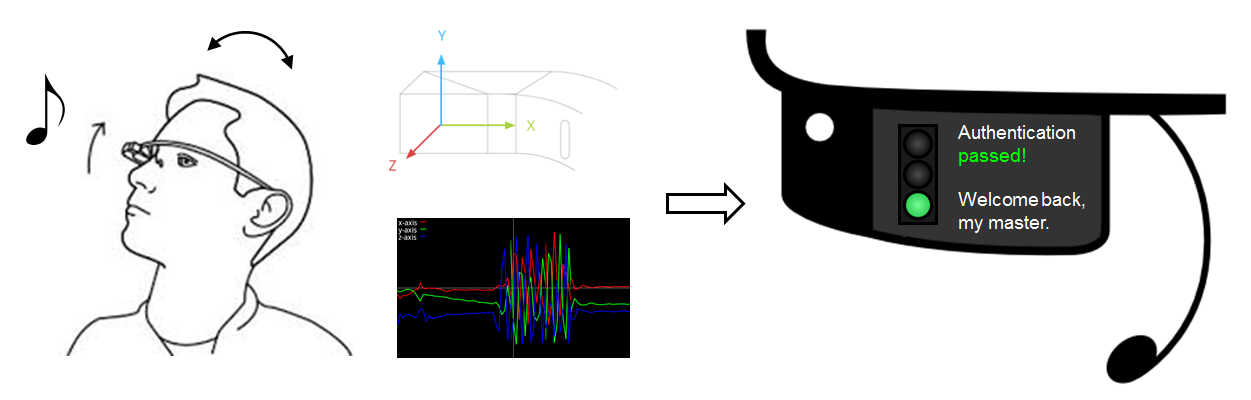
\includegraphics[width=\columnwidth]{fig/headbanger-illustrate.png}
\caption{Illustration of Headbanger. The head-worn device authenticates the
right user based on signatures generated from head-movement patterns in
response to an audio snapshot played on the device.}
\label{fig:headbanger-illustrate}
\end{figure}

\vspace{1mm}\noindent{\bf Authentication Challenge.}
%User-authentication for wearable devices has so-far received relatively less
%attention; commercially as well as in research.
Authentication on most commercially available wearable devices
today~\cite{fitbit, smartwatch} relies on an indirect mechanism, where users
can login to their wearables through their phones. This requires the wearable
device to be registered and paired to the user's mobile device, which makes it
inconvenient as the user has to carry both the devices. The security of this
approach is also in question as it increases the chance of hacking into
 both the devices if either of the devices are lost or stolen.
Some devices including Google Glass~\cite{googleglass} and
FitBit's health tracker~\cite{fitbit}, pair the device to the users email
account instead of the phone for user's convenience; however, it does not add any
security benefit. Though wearable devices today almost contain the same suite
of sensors as a smartphone, the computing capacity and battery lifetime of
wearables are far less comparable. This implies that, translating the same
 authentication solution from a phone to the wearable device, to enable
direct authentication, is not only undesirable but also impractical.
\emph{Thus, the need for the day is a simple, low-power, and accurate
direct authentication solution.}
%For example, fitness trackers and
%smart-watches are tethered to user's mobile device to connect to the
%Internet as well as for remote data collection.

There have also been a few specific point solutions that propose to directly
authenticate the user to the device using biometric signatures~\cite{rahman2014bodybeat,cornelius2014wearable}. However, collecting and recognizing these biometrics is subject
to the availability of the sensing hardware and the computing capability on
the wearable units, hence unrealistic in most
cases. The recent years have also seen a significant interest in using
behavioral characteristics of humans as biometric signatures for mobile phone
authentication~\cite{stevenage1999visual,okumura2006study,monrose2000keystroke,jorgensen2011mouse,bo2013silentsense,de2012touch}.
For example, human walking gait, arm swings, typing patterns, body pulse
beats, eye-blinks have all been found to be distinctive in human beings.
The main advantage of using behavioral biometrics is that the signatures can
be generated from raw data of basic sensor that are inbuilt in mobile phones
such as motion sensors, camera, microphones etc. However, what behavioral
biometric remains the best suited for a wearable device and if such a
biometric can be captured by the wearable device lays a fundamental question
for a system that may adopt this approach.

\vspace{1mm}\noindent{\bf Head-movement based authentication.}
In this paper, we propose to authenticate wearable devices to users based on
their unique behavioral patterns. Keeping in mind the feasibility of
implementation and the availability of the sensor on the wearable device,
we design a system that authenticates users to their device directly through
their head-movement patterns.
In particular, we prototype an authentication system, dubbed {\em Headbanger},
that generates a signature from user's head-movements that serves as the
behavioral biometric for authentication. To ensure that the user is proactive
in making head-movements we stimulate the process by playing a short duration
audio track with fast beats. The user in response to the rhythm and beats
makes head-movements that are captured by the accelerometer and processed to
generate and authenticate the user's unique biometric signature.
While we use a Google Glass a running example for the wearable device, our
design can be applied to other head-worn gadgets and any system that can
record head-movements through motion sensing.
Our choice for using head movements is motivated by the fact that head-worn
wearables are becoming very common today and such devices are already equipped
with motion sensors; for example, personal imaging and heads-up display
devices, gaming headsets, AI devices.

%Unlike physiological biometrics that require custom hardware,
%behavioral biometrics offer a much more available/conveient solution. The
%challenge, however,
%is to ensure that these patterns are repeatable under all circumstances that
%the user encounters as well as the differentiability factor between different
%human beings. %We show that by using the same external stimulus among all
%%users
%the baseline for comparison is achieved much easier and the head-patterns are
%more consistent and differentiable among users.

%Subconscious head-movement, or any body movement as a matter
%of fact, can be very random in general.
% Our design assumes that there is only one owner per glass, and we can easily
%extend our scheme to handle the cases with multiple owners.

In summary, the key contributions of this paper are:

\begin{enumerate}

\item We propose a technique for direct authentication to wearable devices
using head-movement patterns. We show that user's head-movement patterns
contain unique signatures that when inferred correctly can be used as valid
behavioral biometrics for authentication.

\item We design an authentication system, \systemname,~ that records,
processes, generates unique signatures, and classifies head-movement patterns
of users based on the accelerometer (inbuilt on the wearable device) sensor
readings.

\item We devise of a set of light-weight preprocessing and classification algorithms that can effectively transform raw and noisy sensor data into accurate authentication results. We aggressively optimize the processing latencies of these algorithms so that they are well suited for wearable devices.

\item We implement a data collection application on Google Glass that plays a
fast beat music (preloaded) through the Glass's speakers and simultaneously
records and filters accelerometer sensor data. We use this data collection app
in our experiments to evaluate the system.

\item Through extensive experiments involving multiple users\footnote{Our
human user experiments were approved by Rutgers University IRB} and over
different system design parameters we have shown that head-movement patterns
can be used as a
valid behavioral biometric.
To effectively identify a smart wearable device user,
with average false acceptance rate of 4.9\% and average false rejection rate
of 3.9\%.

\item We have conducted detailed validation of using head-movement patterns as a biometric characteristic by collecting and analyzing data from multiple users. We will make these data publicly available, which may facilitate other user behavior studies.
\end{enumerate}

In the sections to follow, we will discuss the background of wearable
device authentication in section~\ref{sec:background} and details of our
proposed system design in section~\ref{sec:design}. We evaluate the system in
section~\ref{sec:results} and follow up with discussions and conclusions in
sections~\ref{sec:disc} and \ref{sec:conc}, respectively.












\iffalse
Wearable devices are typically user-interface constrained
Unlike a smartphone, touch gestures or voice activation or face
recognition units not all wearable devices today have the generic
user interfaces such as touch or audio or visual so that typical
gesture or

The recent years have seen a significant growth in popularity of
smart wearable devices. This growth can be attributed to the advances in
hardware miniaturization technology as well as economically affordable
and energy efficient sensing and computing. While size, energy and cost
constraints remain key motives for improvements in wearable computers'
design, the aspect of user authentication has received relatively less
attention. Wearable devices often collect and store sensitive data about
users, and thus there is an obvious need to authenticate the right user to the
device. Solutions today primarily rely on indirect authentication
mechanisms through the user's smartphone, which can be cumbersome and less
secure. Biometric based solutions, though very effective, however, are subject
to the availability of the specific sensors in the wearable unit. In this
paper, we propose to authenticate wearable devices to users based on their
unique behavioral patterns. In particular, we prototype an authentication
system for wearable devices by monitoring user's unique head-movement patterns
in response to an external audio stimulus. Using a personal imaging device as
a running example, and through extensive experimental evaluation over multiple
users, we show that our mechanism can authenticate users with high accuracy


\fi 